\documentclass[a4paper]{article}

\usepackage[english]{babel}
\usepackage[utf8]{inputenc}
\usepackage{amsmath}
\usepackage{graphicx}
\usepackage{listings}
\usepackage[colorinlistoftodos]{todonotes}
\title{Emergent Architecture Design}
\usepackage{authblk}

\author[1]{Boudewijn van Groos}
\author[2]{Chris Langhout}
\author[3]{Jens Langerak}
\author[4]{Paul van Wijk}
\author[5]{Louis Gosschalk}

\affil[1]{bvangroos \\
4229843}
\affil[2]{clanghout \\
4281705}
\affil[3]{jlangerak \\
4317327}
\affil[4]{pjvanwijk \\
4285034}
\affil[5]{lgosschalk \\
4214528}

\date{\today}

\begin{document}
\maketitle
\tableofcontents
\newpage

\section{Introduction}
This document describes the design of the architecture and it is continuously updated to the current state of the software. It also states the design goals we want to achieve during the project. Furthermore the subsystem decomposition is laid out.

\section{Design goals}

\subsection{Availability}
We will have frequent meetings with the clients. During these meetings we want to be able to show a working prototype of the software in the current state. The feedback provided during the meetings can then be used for improvement. If there are extra features the client wants, we can decide if we will implement them.

\subsection{Modularity}
The program can be split into a number of modules. These modules should be implemented independently of the other modules. Interaction between modules is only possible by making use of defined interfaces. The system is also based on the model-view-controller (MVC) design pattern. See section~\ref{subsec:mvc} for further details on this pattern.

\subsection{Continuous Integration}
There should be always a working product. Each sprint should add one or more features.

\subsection{Understandability}
We must also make the software user-friendly. Even though the users of the
product are already familiar with analysis software, our application should be
easy to learn. It is essential that the user understands the usage of the
scripting language in our application before he/she is able to use it for
analysis.

\subsection{Code quality}
In the project we strive to have good code readability and the code must be easy to understand. This is also an important part of the static analysis. We handle the pull based system on Github. For each new feature that will be implemented the author of that feature must create a new branch and do all his work in that branch so that the master branch always consists of a working version of the software. If someone wants to commit he has to make a pull request first. His code will then be reviewed by at least 2 teammembers and eventually fixed before it can be merged with the working version in the master branch. In addition the code must be diagnosed using static analysis (see section~\ref{sec:static})

\section{Static analysis}
\label{sec:static}
We make use of static analysis tools that provide information about the quality of the software:
\begin{description}
\item[Corbertura] We use this tool to find out how much test coverage we have in our system. Our goal is to keep the line coverage as well as the branch coverage at at least 75\%. This means that not only cases where the program works well should be tested, but also the cases where the program should fail.
\item[Checkstyle] To improve code quality in terms of styling we have code conventions which the writer should follow before his code is accepted. This is done by the Checkstyle plugin in the IDE that makes sure these conventions are followed.
\item[FindBugs] This tool will help us find where our program may contain some faults. This also makes code reviewing for teammembers easier since the process is automated. If there are faults, the writer should fix them to make the code acceptable.
\item[PMD] The program can contain some programming mistakes such as unused imports or dead code. Since we do not want these mistakes in the code we use PMD to detect these mistakes using PMD's built-in rules.
\end{description}

It is up to the writer to fix the warnings produced by these tools, or provide a clear explanation whether the warning will not be fixed.


\section{Software architecture views}

\subsection{Model View Controller}
\label{subsec:mvc}
The software is based on the model-view-controller design pattern. The idea is that we want the analyis data in the columns (model) separated from the user interface (view). The interaction between these modules will be accomplished with the controller module. The controller is able to change the view and uses data that is obtained from the model. The user will be able to modify the model by providing operations to the controller which will then change the model.

\subsection{Subsystem decomposition}

As mentioned before our program consists of modules that work together. In figure~\ref{fig:modules} these modules are laid out. We realized that the structure we have now does not entirely fit the MVC pattern since there are modules that are not really a part of the MVC. We will change the structure in the near future in a way that each model is a part of a module in the MVC.

\begin{figure}[h]
	\centering
    	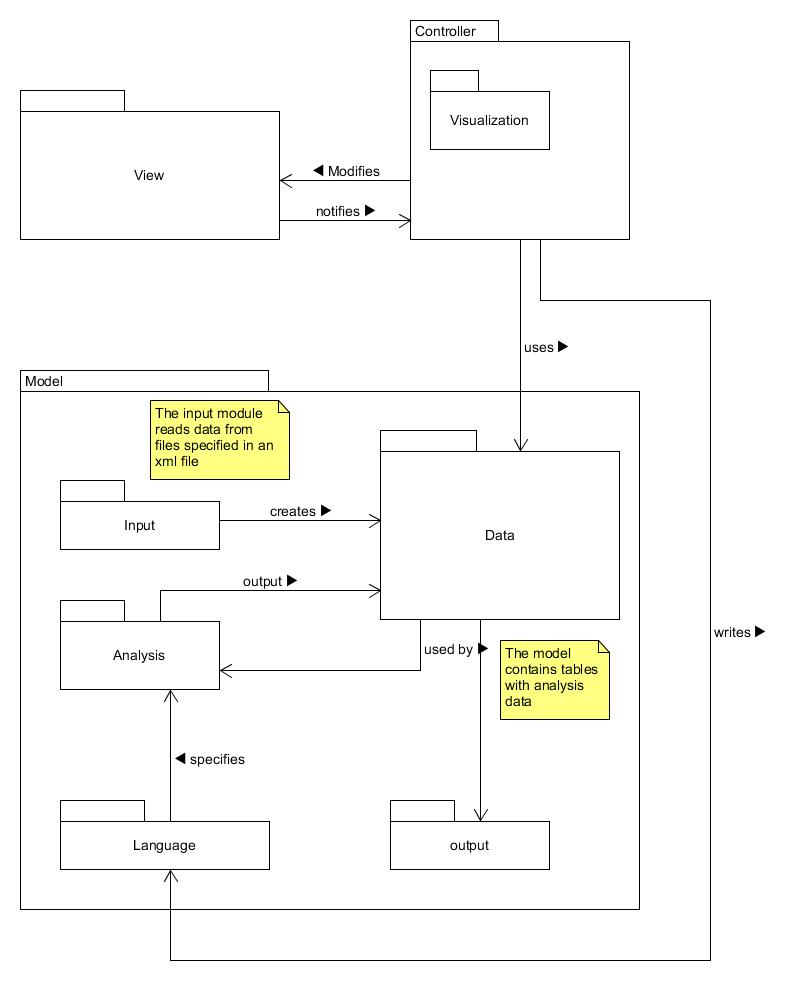
\includegraphics[scale=0.5]{images/modules.jpg}
    \caption{Modules of the system}
	\label{fig:modules}
\end{figure}

\begin{description}
\item[Input]
The input module is able to read the data from provided files that are specified in an xml file. With that data a dataModel can be constructed.
\item[Model]
The model module contains and manages the data that was read and/or analyzed by the user. This data will also be provided to the controller and analysis modules. The data is stored in tables. 
\item[Analysis Specification]
The Analysis Specification module processes the SUGAR script that defines how the data should be analyzed. The user provides this script. In this module the script is parsed in operations that can be performed by the Analysis Module.
\item[Analysis]
The Analysis Module performs the analyses over the dataModel. It contains all the operations (the 8 C's) to make the exploratory sequential data analysis possible. The output of this module is the result of the analysis, this is a table that will be added to the model.
\item[Controller]
The controller module is responsible for the program's front-end behaviour. It is the module to which the user has access. The controller uses the current state of the model to produce the according view for the user.
\item[Visualization]
The Visualization module creates a certain visual representation of a dataModel. For example it can create a box-plot of the creatine levels. The visualization is kept up to date by the controller if the data changes.
\item[View]
The view module is responsible for the appearance of the user interface. Determining by the controller, the view can change accordingly. The user may change the view after which the controller gets notified. The controller can then perform actions on the model.

\end{description}
\subsection{State diagram}
Figure~\ref{fig:statemachine} represents the state diagram which describes the flow of the program.
\begin{figure}[h]
	\centering
	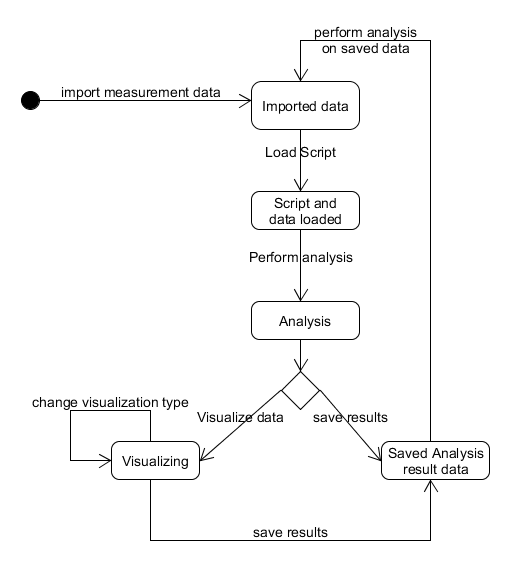
\includegraphics[scale=0.5]{images/statemachine.png}
	\caption{State diagram of the program}
	\label{fig:statemachine}
\end{figure}

\section{Software architecture}

\subsection{Programming languages and auxiliary programs}
The software will mainly be written in Java since this was obligatory in
the project. For the graphical user interface we make use of the JavaFX
framework and is written using fxml. We use Eclipse and IntelliJ IDEA as IDE to
write the Java code with. 
For continuous integration and version control we use Git and Github. Locally we use Maven to build the project. On GitHub we use Travis CI to verify the builds.
We also use the JavaFX Scene Builder as a tool to design parts of the GUI because this provides a better preview of what the interface will look like while creating it.

\subsection{Used libraries}
\begin{description}

\item[JavaFX] Creating the graphical user interface. We mainly chose JavaFX because it is already included in Oracle's Java 8 and provides some
improvements on Oracle's previous frameworks. One of these is the use of fxml to
construct the static part (view) of the GUI. The advantage of fxml is that this static part is separated from the controller part so we do not have cluttered up code and long methods just to build up a window. Some of us already gained some
experience with it during the Software Engineering Methods course.

\item[Mockito] Mocking objects to test behavior. We did not specifically choose
for this framework but we have used it before in previous courses and it did not
seem like a big necessity to change to a different mocking framework as this
will only require more effort to learn it.

\item[Apache POI] Reading data analysis files stored in the Microsoft Excel
format. This is one of the main excel parsers and easy to use. We chose this
library because it applies very good solution for reading the data that was
provided to us in excel formats. Another reason is that it is developed by the 
Apache Software Foundation which also created Maven so it was easy to include in
the build.

\item[Java SAX] Reading the xml file that specifies the datafiles. This choice is
made because it is easy to use and well documented. The library is also included
in the JDK so it did not require any additional installation effort.

\item[Parboiled] In the parser department we had lots of choice. We tried to find a
framework which was both simple to use and still powerful enough for our use. This lead
us to Parboiled. The beauty of Parboiled is the fact that you can write your rules in
plain Java. This means you don't get an extra build process. The disadvantage is that
Parboiled does some magical stuff which our analysis tools don't fully understand, 
so you need to be aware of it. All in all we're really satisfied with the strength of
Parboiled and feel that we've made the right choice.

\end{description}

\section{Testing}
\subsection{Unit testing}
To make sure that all the code works as it should, the author must always write
unit tests for the code he has written. We make use of the JUnit framework to
write the tests. To verify behaviour of methods we use the Mockito framework to
stub certain object needed by the method.

\section{Glossarium}

\begin{description}

\item[Analysis] An analysis that can be done on measuring data to come to an answer to a specific question.
\item[Git \& GitHub] Git is the tool to control the versions in a repository. GitHub is the web-tool to make the versions available for group use.
\item[GUI] Graphical User Interface.
\item[IDE] Integrated Development Environment.
\item[JDK] Java development kit.
\item[MVC] The Model-View-Controller design pattern.
\item[SUGAR] The scripting language used to create analyses.
\item[Pull Request] Are made on GitHub to get your commits to the code verified and merged with the master branch.

\end{description}

\end{document}
